\begin{frame}
  \frametitle{\textbf{The Standard Model of Particle Physics}}
  \begin{columns}
    \column{0.65\textwidth}
    \begin{tikzpicture}
      \node{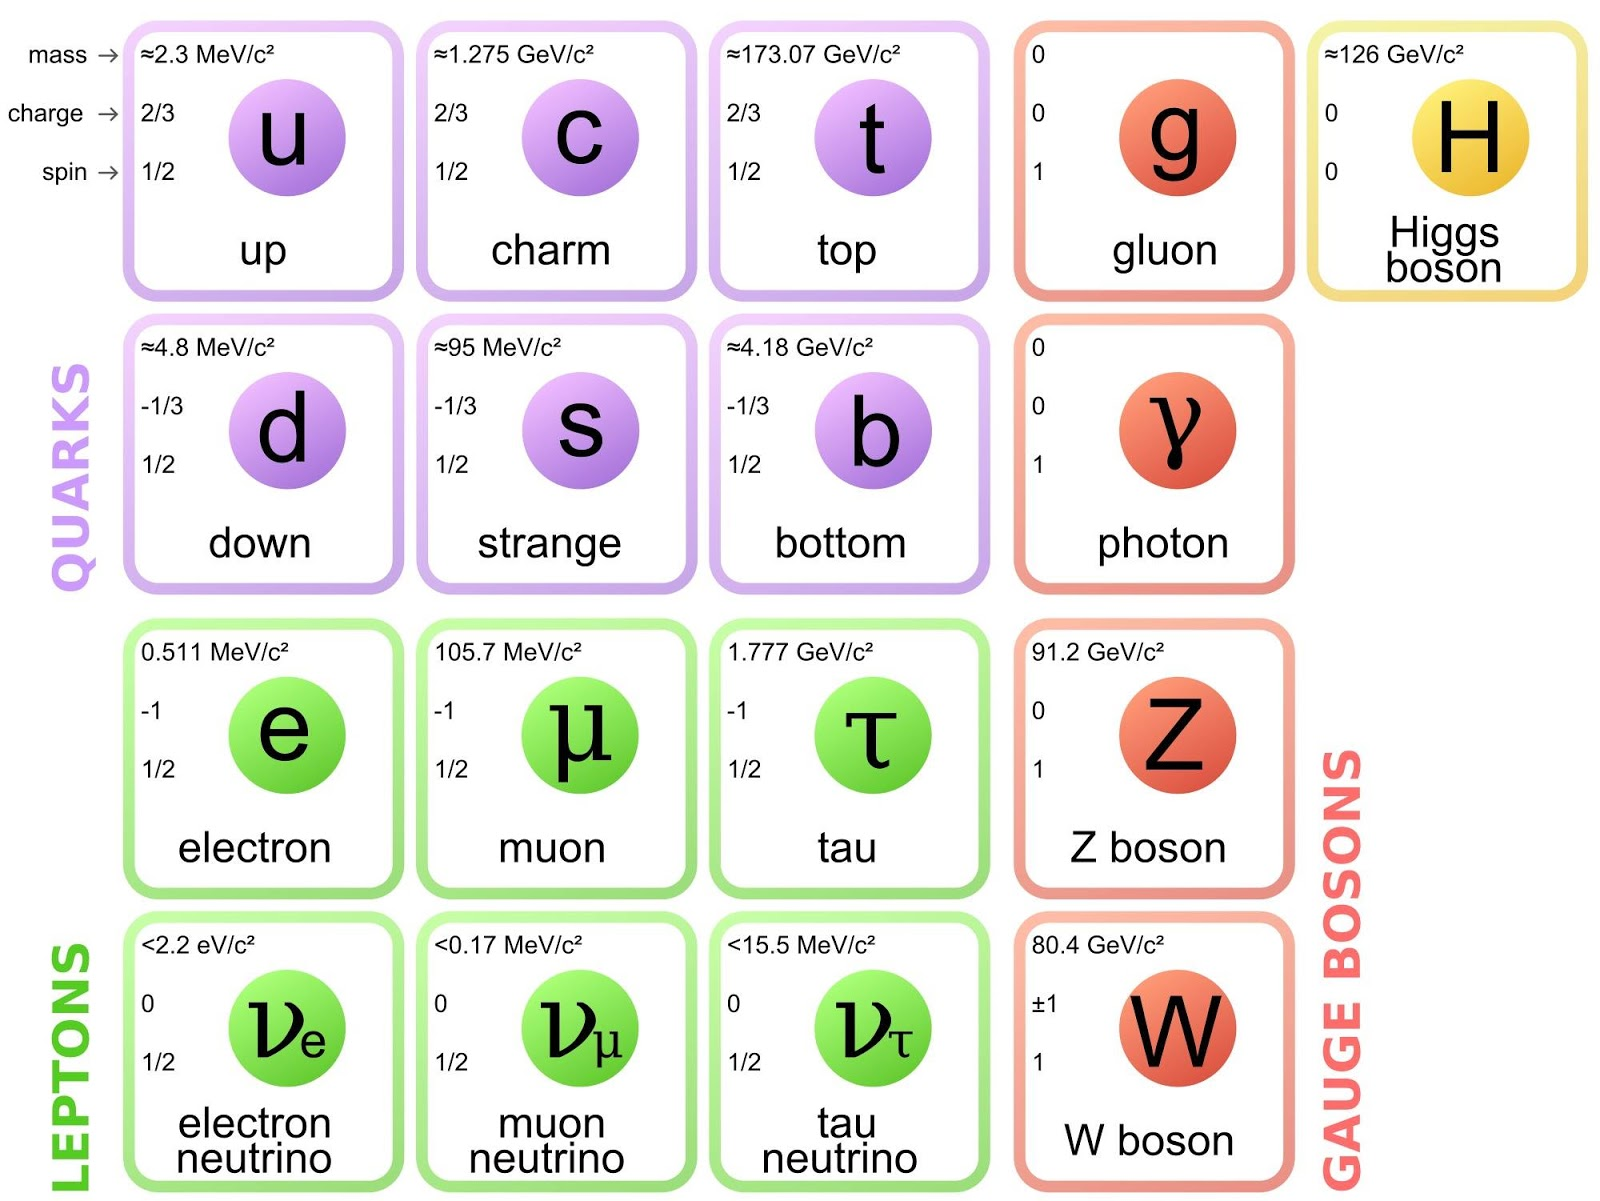
\includegraphics[width=\textwidth]{standard-model.jpg}};
      \node[font=\tiny] at (-1.5,-3.2) {\href{https://en.wikipedia.org/wiki/Standard_Model}{https://en.wikipedia.org/wiki/Standard\_Model}};
    \end{tikzpicture}
    \column{0.35\textwidth}
    \begin{itemize}
    \item Quantum field theory that describes
      \begin{itemize}
      \item Quantum electrodynamics
      \item Electroweak interactions
      \item Quantum chromodynamics
      \item \st{Gravity}
      \end{itemize}
    \item Quarks and leptons interact via the exchange of gauge bosons
      \begin{itemize}
      \item QED $\to \gamma$
      \item EW $\to W^{\pm}, Z$
      \item QCD $\to g$
      \end{itemize}
    \item $H$ is a mass-giving scalar boson
    \item \textbf{Experimentally verified}
    \item Still open questions...
      \begin{itemize}
      \item muon $g-2$ anomaly
      \item non-zero neutrino mass
      \item baryon asymmetry
      \end{itemize}
    \end{itemize}
  \end{columns}
\end{frame}

